\documentclass[11pt]{beamer}
\usetheme{Warsaw}
\usepackage[utf8]{inputenc}
%\usepackage[magyar]{babel}
\usepackage[T1]{fontenc}
\usepackage{amsmath}
\usepackage{amsfonts}
\usepackage{amssymb}
\usepackage{graphicx}
\usepackage{xurl}
\usepackage{multimedia}
\usepackage{xurl}
\newenvironment{trienv}{\only{\setbeamertemplate{items}[triangle]}}{}
\newenvironment{squareenv}{\only{\setbeamertemplate{items}[square]}}{}
\author{Bendegúz Borkovits T7UR9P}
\title{Simulating detectors with Geant4 3rd presentation}
%\setbeamercovered{transparent} 
\setbeamertemplate{navigation symbols}{\insertframenumber/\inserttotalframenumber} 
%\logo{} 
\institute{Scientific Modeling Computer Laboratory} 
\date{April 2022} 
%\subject{} 
\begin{document}


\begin{frame}
\titlepage
\end{frame}

\begin{frame}{Previously...}
    \begin{figure}
        \centering
        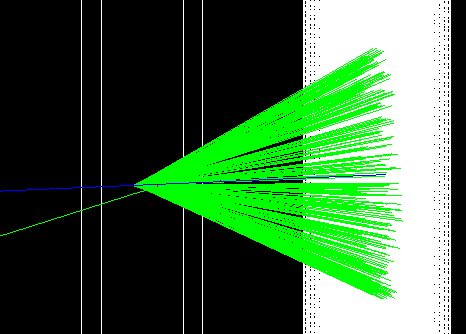
\includegraphics[scale = 0.8]{sensitive_detectors.png}
    \end{figure}
    \begin{itemize}
        \item<tri@1-> Cherenkov detector simulation.
        \vspace{0.2 cm}
        \item<tri@1-> Showcasing the output.
        \vspace{0.2 cm}
        \item<tri@1-> Saving data and analysis in Python.
    \end{itemize}
\end{frame}

\begin{frame}{NEBULA detector}
    \begin{itemize}
        \item<tri@1-> Scintillator array with large volume.
        \item<tri@1-> Fast neutron events in range 100-300 MeV.
        \item<tri@1-> Part of SAMURAI beam line at RIKEN RI Beam Factory.
        \item<tri@1-> 120 NEUT and 48 VETO detector modules (2-layer walls).
        \item<tri@1-> Modules contain a plastic scintillator and 2 PMTs.
    \end{itemize}
    \begin{figure}
        \centering
        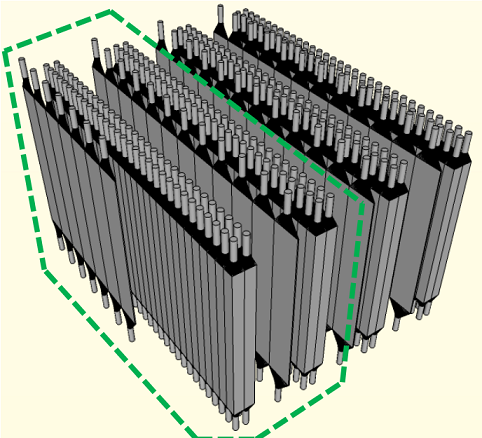
\includegraphics[scale = 0.6]{walls.png}
    \end{figure}
\end{frame}

\begin{frame}{NEBULA detector}
    \begin{figure}
        \centering
        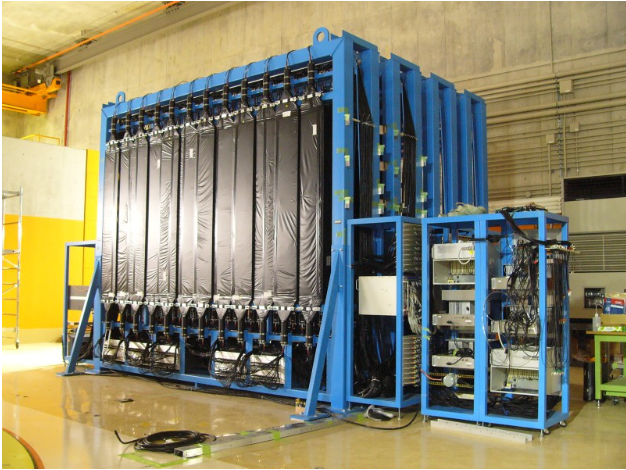
\includegraphics[scale = 0.8]{nebulakep.png}
    \end{figure} 
\end{frame}

\begin{frame}{Smsimulator}
    \begin{itemize}
        \item<tri@1-> NEBULA simulator.
        \vspace{0.2 cm}
        \item<tri@1-> C++ program based on Geant4.
        \vspace{0.2 cm}
        \item<tri@1-> ROOT libraries for visualisation.
        \vspace{0.2 cm}
        \item<tri@1-> Updated frequently.
        \vspace{0.2 cm}
        \item<tri@1-> Offers the following:
        \vspace{0.2 cm}
        \begin{itemize}
            \item<square@1-> simulating response to a single neutron,
            \vspace{0.2 cm}
            \item<square@1-> simulating trajectory of charged fragment in the SAMURAI magnet,
            \vspace{0.2 cm}
            \item<square@1-> simulation for N-body neutron decay.
        \end{itemize}
        \vspace{0.2 cm}
        \item<tri@1-> Very difficult to install.
    \end{itemize}    
\end{frame}

\begin{frame}{Solution and further plans}
    \begin{itemize}
    \item<tri@1-> Solution:
    \vspace{0.2 cm}
    \begin{itemize}
        \item<square@1-> Simulation made by Balázs Pál.
        \vspace{0.2 cm}
        \item<square@1-> Modifications.
        \vspace{0.2 cm}
        \item<square@1-> Programming error: consultation is still underway.
    \end{itemize}
    \vspace{0.2 cm}
    \item<tri@1-> Plans for the next weeks:
    \vspace{0.2 cm}
    \begin{itemize}
        \item<square@1-> Neutron with energy of 100 MeV.
        \vspace{0.2 cm}
        \item<square@1-> Output showcase.
        \vspace{0.2 cm}
        \item<square@1-> Statistical analysis.
    \end{itemize}
    \end{itemize}
\end{frame}

\begin{frame}{References}
    \begin{itemize}
        \item<tri@1-> Geant4 documentation: \url{https://geant4.web.cern.ch/}
        \vspace{0.2 cm}
        \item<tri@1-> NEBULA detector official site: \url{http://be.nucl.ap.titech.ac.jp/~nebula/index.php}
        \vspace{0.2 cm}
        \item<tri@1-> Smsimulator official site: \url{http://be.nucl.ap.titech.ac.jp/~nebula/simulator.php}
        \vspace{0.2 cm}
        \item<tri@1-> RI Beam factory informations: \url{https://www.riken.jp/en/collab/resources/ribf/}
        \vspace{0.2 cm}
        \item<tri@1-> Balázs Pál simulation: \url{https://github.com/masterdesky/ELTE_Modelling_Lab_2021/tree/main/project/project_nebula/NEBULA}
    \end{itemize}
\end{frame}



\end{document}
